\documentclass{article}
% MGPA merged_v5: principle, theory, two constructions and aligned experiments.
% Main evidence: controlled, recorded EEG and P300-selected cross-task reuse.
% Presentation assets are generated from archived results without refitting.
% Historical sources and reference results remain unchanged.
\usepackage[T1]{fontenc}
\makeatletter
\def\input@path{{iclr2027/}}
\makeatother
\usepackage{microtype,graphicx,booktabs,longtable,array,multirow,xurl,placeins,float}
\floatstyle{ruled}
\newfloat{algorithm}{tbp}{loa}
\floatname{algorithm}{Algorithm}
\usepackage{iclr2027/fancyhdr}
\usepackage{natbib}
\usepackage{iclr2027_conference,times}
\usepackage{amsmath,amssymb,amsthm}
\usepackage{xcolor}
\usepackage{hyperref}
\usepackage[capitalize,noabbrev]{cleveref}
\crefname{algorithm}{Algorithm}{Algorithms}
\theoremstyle{plain}
\newtheorem{theorem}{Theorem}
\newtheorem{proposition}[theorem]{Proposition}
\newtheorem{corollary}[theorem]{Corollary}
\newtheorem{lemma}[theorem]{Lemma}
\theoremstyle{definition}
\newtheorem{definition}[theorem]{Definition}
\newcommand{\R}{\mathbb R}
\newcommand{\E}{\mathbb E}
\newcommand{\I}{\mathsf I}
\newcommand{\KL}{\mathrm{KL}}
\newcommand{\method}{\textsc{MGPA}}
\newcommand{\impl}{\textsc{MGPA-Iter}}
\newcommand{\sg}{s_Q}
\DeclareMathOperator{\logit}{logit}
\DeclareMathOperator{\Cov}{Cov}
\DeclareMathOperator{\Var}{Var}
\DeclareMathOperator{\tr}{tr}
\DeclareMathOperator{\range}{range}
\DeclareMathOperator{\diag}{diag}
\makeatletter
\newcommand{\tablerows}[1]{\@@input#1 }
\makeatother
% Keep floats flexible; reserve float-only pages for substantially filled pages.
\renewcommand{\floatpagefraction}{0.85}
\title{Measurement-Gated Provenance Attenuation\\for Frozen EEG Representations}
\author{}
\hypersetup{colorlinks=true,linkcolor=black,citecolor=black,urlcolor=blue!55!black,
pdfauthor={Anonymous authors},pdftitle={Measurement-Gated Provenance Attenuation for Frozen EEG Representations}}
\begin{document}
\maketitle
% Keep the template's nominal spacing; leave surplus space at the page foot.
\raggedbottom
% ===== 00_abstract.tex =====
\begin{abstract}
Frozen EEG representations can encode both neural activity and
signatures of the acquisition pipeline. Source predictability alone does not
identify what should be removed: it can reflect measurement effects or
genuine biological and population differences. We study how measurement
calibration can guide reusable correction of a pretrained encoder's
representations on downstream datasets, without retraining the encoder.
We introduce
Measurement-Gated Provenance Attenuation (MGPA), a framework for selective,
measurement-informed correction. Paired measurement contrasts define an
editable subspace without requiring its wholesale removal. Correction targets
account for source information in the coordinates left unchanged.
For exact affine score matching, we show that different
targets retain the same information at different movement costs, and that
the conditional mean source score given the preserved coordinates minimizes
expected cost within the analyzed class.
We realize this principle in two complementary forms: Closed-form MGPA
estimates a single analytic correction from measurement pairs, while
Iterative MGPA uses learned nonlinear source critics. Both apply to
individual representations without source identity at deployment. Controlled
comparisons show stronger source attenuation with measurement-derived edit
spaces than with rank-matched PCA and random subspaces at matched movement
budgets. On real EEG recordings, Iterative MGPA reduces source accessibility
while maintaining or improving observed task performance; a critic ablation
demonstrates the additional value of nonlinear correction.
Adapters fitted and selected on P300 improve the robustness of frozen N170
and MMN heads under device--label association shifts without target-task
adapter tuning. Separate control-head performance remains close to identity.
\end{abstract}
% ===== 01_introduction.tex =====
\section{Introduction}
\label{sec:introduction}
Frozen EEG foundation models enable lightweight transfer when labeled
data are scarce \citep{wang2024eegpt}, but freezing also preserves
acquisition sensitivities already encoded in their representations.
We ask how measurement calibration can guide reusable correction of these
representations on downstream data, without retraining the encoder.
Physiological waveforms are measurements, not direct observations of physiology.
Reference, montage, channel configuration, preprocessing, and recording
workflow can all alter the signal presented to the encoder
\citep{nunez2006,dong2019}. Acquisition signatures can help reconstruct
a recording without being the physiological evidence a downstream task
seeks.

When recording source (such as the acquisition device or preprocessing
condition) correlates with a downstream label, a lightweight head may
exploit these cues rather than task-relevant neural information.
Strong average performance can conceal this shortcut until
the source--target association changes \citep{geirhos2020}, as related
failures in multi-site clinical prediction illustrate \citep{zech2018}.
Such failure need not require an unseen device: changing how familiar
acquisition conditions co-occur with the target can invalidate the same
predictor. A source probe establishes accessibility, not whether a task
head uses that channel. Moreover, source can be associated with genuine
biological or population differences. Indiscriminate source erasure can
therefore discard the very variation a downstream task needs
\citep{yamashita2019}.

\begin{figure}[htbp]
\centering
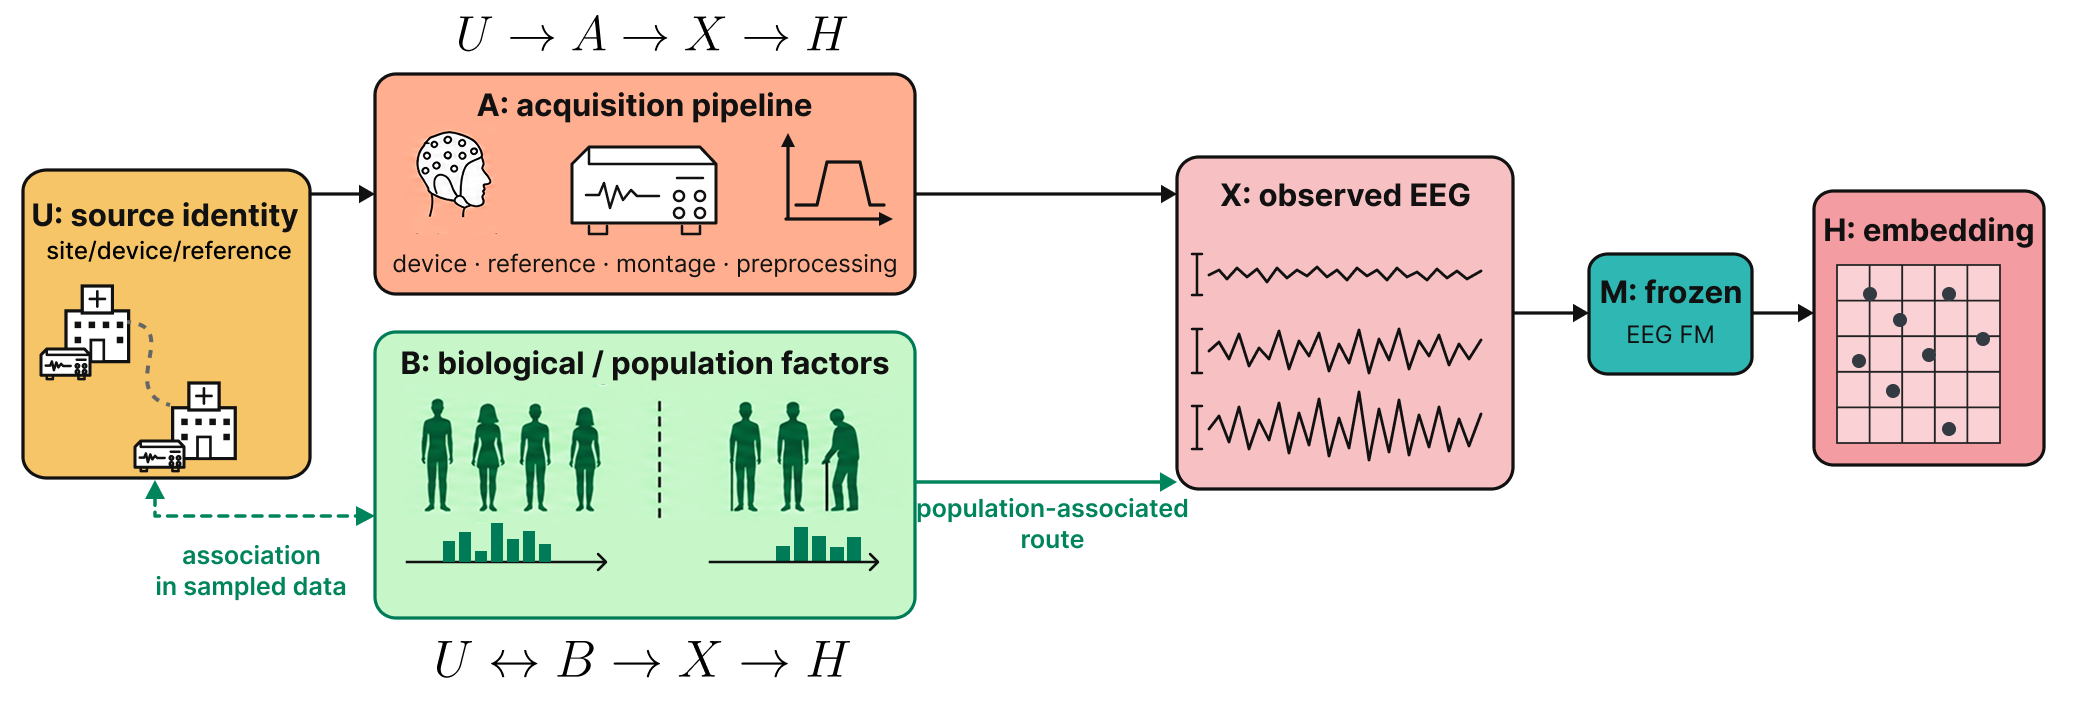
\includegraphics[width=\linewidth]{assets/measurement_paths.png}
\caption{\textbf{Two routes to source-predictive frozen EEG representations.}
Source predictability can arise through measurement $A$ or sampling
association with biological/population factors $B$. Here $U$ denotes source,
$X$ observed EEG, and $H=M(X)$ its representation from frozen encoder $M$.
Symbols are local to this diagram.}
\label{fig:measurement-paths}
\end{figure}

Source-labeled representations alone cannot generally separate the two
routes in Figure~\ref{fig:measurement-paths}. Measurement contrasts supply different
evidence: they compare representations of the same underlying observation
under specified measurement changes. Examples include applying different
references to a stored EEG trial and observing a shared event with simultaneous
recording systems. Such calibration provides evidence about which representation
directions respond to measurement changes, rather than merely distinguish
source groups.

We introduce \emph{Measurement-Gated Provenance Attenuation} (\method),
a principle and construction for selective correction of fixed representations.
Its \emph{measurement gate} restricts edits to a fixed subspace defined by
measurement contrasts. The remaining coordinates $Q$ stay unchanged.
The gate permits changing a direction but does not require deleting it.
Measurement-sensitive coordinates may still contain variation useful to
downstream tasks. MGPA separates where measurement evidence permits a change
from how each observation should move within that space.

We instantiate this principle in two complementary forms. \emph{Closed-form MGPA}
estimates a correction direction from paired measurement contrasts and applies
one analytic adjustment to each representation. \emph{Iterative MGPA} fits
predictors of recording source, called \emph{critics}, and uses their scores to
guide small, bounded steps within the permitted subspace. Critics are refitted
as representations change: \emph{the critic proposes, and the intervention
constrains}. Both implementations leave $Q$ unchanged.

This leaves a shared question: what should correction target when $Q$ remains
unchanged? Suppose a predictor using $Q$ alone assigns probability $.8$ to one
of two equally likely sources. Editing the other coordinates cannot remove
that retained evidence. Forcing a predictor using the full representation to
output $.5$ instead asks editable coordinates to counteract evidence still
available in $Q$.

Our analysis separates retained information from correction cost.
For a fixed source score affine in the editable coordinates and a fixed
correction metric, exact matching to different targets determined by $Q$
preserves the same information at different movement costs. Expected cost
is minimized by the conditional mean: the expected source score given $Q$,
not the probability of source given $Q$. Both implementations estimate this
conditional-mean target.

At fixed hyperparameters, both implementations are fitted using measurement
calibration and source labels, without downstream task labels. In our reuse
experiment, correction strength is selected using P300 development labels and
held fixed across the other tasks. At deployment, the fitted map corrects
individual representations without changing their dimension or requiring source
identity, paired observations, or encoder retraining. The construction applies
to fixed representations, including pretrained EEG embeddings and conventional
EEG features.

\paragraph{Contributions.}
First, we formulate MGPA, combining measurement-supported edit permissions
with selective correction that preserves a fixed complement. Second, we
establish cost-optimal conditional-mean anchoring within the analyzed class of
exact affine score-matching corrections and characterize Gaussian selective
erasure, including residual source separation under direction error.
Third, we develop Closed-form MGPA and
Iterative MGPA, two complementary implementations with source-blind deployment.
Finally, we test selective correction, nonlinear critics and cross-task reuse
in complementary controlled and recorded-data protocols.
Table~\ref{tab:results-glance} previews the empirical evidence before the
formal construction; Section~\ref{sec:experiments} develops the full comparisons.

\begin{table}[htbp]
\centering\small
\caption{\textbf{Main experimental questions and findings.}
Source AUROC: lower is better;
task AUROC: higher is better. Arrows compare identity with MGPA;
row 3 reports gains over LEACE. Full comparisons and paired intervals are in
Sections~\ref{sec:gate-result}--\ref{sec:recovery}.}
\label{tab:results-glance}
\begin{tabular}{@{}>{\raggedright\arraybackslash}p{\dimexpr.45\linewidth-\tabcolsep\relax}>{\raggedright\arraybackslash}p{\dimexpr.55\linewidth-\tabcolsep\relax}@{}}
\toprule
Research question and construction & Empirical preview \\
\midrule
\textbf{Can measurement-related source information be attenuated without losing task utility?}\newline
Controlled SSVEP; Closed-form MGPA &
Source AUROC: $.683\to .510$.\newline
Task AUROC, head unchanged: $.7528\to .7526$. \\
\addlinespace
\textbf{Does selective correction remain useful on real recordings?}\newline
Temporal N170 and recorded wet/dry SSVEP; Iterative MGPA &
\textbf{N170:} source AUROC $.989\to .946$;\newline
refitted-task AUROC $.728\to .746$.\newline
\textbf{SSVEP:} source AUROC $.916\to .872$;\newline
refitted-task AUROC $.688\to .689$. \\
\addlinespace
\textbf{Can a correction selected on one task improve shortcut robustness on other tasks?}\newline
P300-selected Iterative MGPA &
Frozen-head AUROC gains over LEACE at the worst device--label association:\newline
$+.057$ on N170 and $+.019$ on MMN. \\
\bottomrule
\end{tabular}
\end{table}

% ===== 02_related_work.tex =====
\section{Related Work}
\label{sec:related}

\paragraph{Concept erasure and conditional invariance.}
INLP removes linearly predictive directions through repeated nullspace
projection \citep{ravfogel2020}; LEACE gives a closed-form, minimum-distortion
affine eraser with linear guardedness \citep{belrose2023}.
Closed-form MGPA also yields an affine map, but estimates its correction
direction from paired measurement contrasts and conditions its target on the
coordinates preserved by the gate. IGBP extends
erasure to nonlinear decision surfaces through iterative critic refitting
\citep{iskander2023}, while MANCE restricts nonlinear edits to local tangents
of the natural representation manifold \citep{avitan2026mance}.
MGPA separates measurement-supported edit permissions from the correction
rule: a source-predictive direction alone does not authorize its removal.
This also differs from preserving covariance with a supplied task
label, as in SPLINCE \citep{holstege2025splince}. CIRCE learns nuisance
independence conditional on task information \citep{pogodin2023circe},
and conditional probing measures information beyond a baseline
\citep{hewitt2021conditional}. In MGPA, the conditioning variable is the
complement fixed by the measurement gate. Our analysis separates retained
information from coordinate distortion, and its Gaussian specialization
connects conditional-mean anchoring to minimum-distortion linear erasure.

\paragraph{Measurement harmonization and EEG transfer.}
Traveling-subject designs distinguish measurement bias from population
sampling bias \citep{yamashita2019}. Noisy Counterfactual Matching estimates
a subspace from paired differences and removes it by projection
\citep{bai2025ncm}. MGPA instead uses measurement contrasts to constrain
selective edits. Several alignment methods need no target-task labels: CORAL
matches domain covariances \citep{sun2016coral}, Euclidean alignment
normalizes EEG covariance \citep{he2020ea}, and CMMN aligns spectral
distributions \citep{gnassounou2023}. Riemannian Procrustes combines
geometric alignment with a class-informed rotation
\citep{rodrigues2019rpa}. AwAR and SDDA address cross-headset classification
through adaptation regularization and spatial distillation/distribution
alignment, respectively \citep{wu2016awar,liu2026sdda}.
Both MGPA implementations operate on fixed representations, require no
downstream labels during fitting at fixed settings, and apply a stored
correction to individual representations without source identity.

\paragraph{Paired and post-training embedding adapters.}
FEATMAP is a close acquisition-harmonization predecessor: paired
measurements train a reusable affine map between medical foundation-model
embedding domains without downstream labels \citep{donle2026featmap}.
Post-Training Augmentation Invariance learns lightweight adapters on
frozen representations while approximately preserving the geometry of
unaugmented features \citep{eikenberry2026}; PISCO separates style and
content in pretrained representations \citep{ngweta2023}. These works
establish reusable post-training correction; MGPA specifies which changes
calibration supports and how to perform them while retaining the fixed
complement. MGPA links measurement-supported edit constraints to target choice.
Closed-form MGPA implements this construction analytically; Iterative MGPA
uses refitted source critics and bounded trust-region updates.
Iterative MGPA's local trust-region solve uses classical
optimization machinery \citep{more1983}. Our comparisons
distinguish edit permissions, calibration inputs and deployment routing,
as well as source attenuation and downstream utility.
% ===== 03_problem_and_gate.tex =====
\section{The MGPA Principle: Measurement-Supported Correction}
\label{sec:admissibility}
\paragraph{Fixed representations and measurement contrasts.}
Let $H\in\R^d$ be a representation produced by a frozen encoder or a fixed
feature extractor. Its source $U\in\{0,1\}$ indexes an acquisition system
or a constructed measurement view; $Y$ denotes a downstream task.
Calibration data include paired representations $H_i^{(a)},H_i^{(b)}$:
either two specified transformations of the same stored trial or observations
of the same unit under different acquisition conditions. A same-unit contrast
supplies evidence about measurement response beyond observational source prediction.
Assume paired views share a content contribution and have additive measurement
responses in a fixed subspace. Their contrast
$\Delta_i^{ab}=H_i^{(a)}-H_i^{(b)}$ cancels the shared contribution; the remaining
response may depend on content in both magnitude and direction. Recovering the
full response span requires calibration contrasts that span it \citep{bai2025ncm}.

\paragraph{A fixed complement, not wholesale deletion.}
Let $B\in\R^{d\times r}$ have orthonormal columns spanning the directions
supported by calibration. The \emph{measurement gate} $P=BB^\top$ restricts
edits to their span. This constraint does not separate exclusively biological
from instrumental coordinates. Let $Z=B^\top H$ be editable coordinates and
$Q=q(H)=(I-P)H$ the fixed complement. Admissible corrections have the form
\begin{equation}
 R(h)=q(h)+B\psi(h),
 \label{eq:admissible}
\end{equation}
where $\psi(h)\in\R^r$ contains the corrected editable coordinates.
Thus $Q$ is recoverable from every admissible output. Conditioning on the
fitted gate, the information chain rule gives
\begin{equation}
 \I\{U;R(H)\}=\I(U;Q)+\I\{U;R(H)\mid Q\}.
 \label{eq:floor}
\end{equation}
The first term is fixed by the admissible class. It can be nonzero through
source-associated content or measurement variation outside the fitted gate;
balanced source counts alone do not make the complement source-independent.
The editable coordinates can also contain useful task variation, so permission
to change them is not an instruction to discard them. This defines the
correction problem: change selected components of $Z$ while retaining $Q$.

\paragraph{A measurement-gate estimator.}
We estimate the measurement gate using normalized-contrast SVD. Fit-only
preprocessing establishes shared featurewise-standardized coordinates.
Each retained nonzero contrast $\Delta_i^{ab}$ is normalized to unit length.
This makes the estimated subspace reflect recurring directions of measurement
change rather than the magnitude of individual displacements.
Stack these normalized contrasts as rows of $D_A$
and compute its thin singular-value decomposition:
\begin{equation}
 D_A=L_A\Sigma_AV_A^\top,\qquad
 B=[v_1,\ldots,v_r],\quad P=BB^\top.
 \label{eq:gate-estimate}
\end{equation}
The retained rank $r$ is set by a retained-energy criterion or selected on
development data, as specified by the experimental protocol. The gate remains
fixed throughout fitting and deployment of the correction; a zero-rank gate
returns identity. Appendix~\ref{app:protocols} specifies contrast construction,
preprocessing, numerical filtering and rank selection.

\paragraph{From edit permission to provenance correction.}
The gate specifies where correction may act, but leaves its target and update
rule to be chosen. We next study how targets determined by $Q$ affect retained
information and movement for a fixed affine source score. This analysis
motivates the score's conditional expectation given $Q$ as a reference; for
affine scores, that expectation can be obtained from $\E[Z\mid Q]$.
% ===== 05_target_analysis.tex =====
\section{Why the Gate Changes the Target}
\label{sec:targets}
Figure~\ref{fig:theory-geometry} previews three choices: where edits are
permitted, how much of the editable block to replace, and where to place
the result. The gate fixes the first; we now study the other two.

\begin{figure}[htbp]
\centering
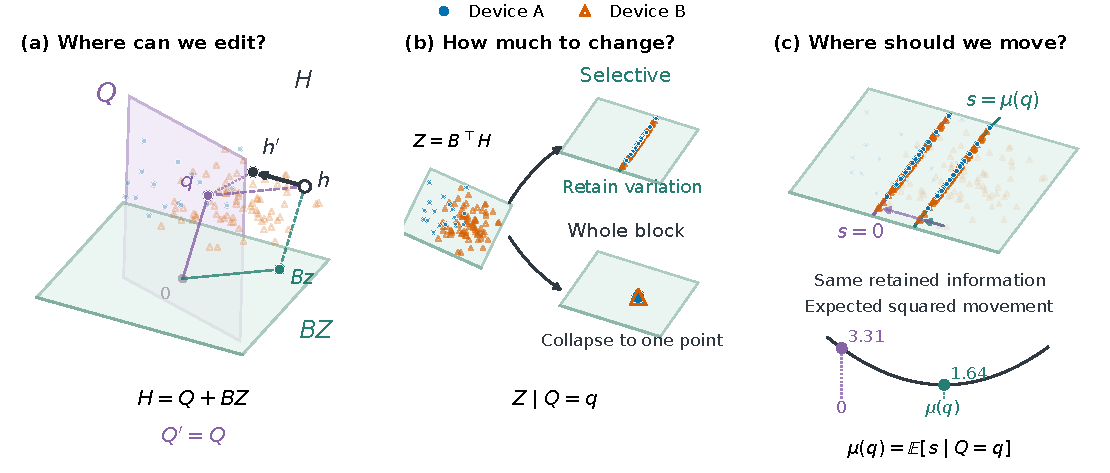
\includegraphics[width=\linewidth]{assets/theory_story.pdf}
\caption{\textbf{Three choices in measurement-gated correction.}
(a) Full embeddings $H=Q+BZ$: dashed guides show component projections;
the black arrow edits $BZ$ while preserving $Q$. The subspaces are orthogonal
before the display projection.
(b) At fixed $Q=q$, selective correction retains variation lost by replacing
the whole editable block.
(c) In the same conditional slice, two score targets retain the same information at different expected
movement costs; the minimum is at the conditional-mean score $\mu(q)$.
In this Gaussian illustration, $Z$ has source means $(\pm1,0)$, covariance
$I_2$, and $\Pr(B\mid q)=.8$, giving $s=\log4+2z_1$.
Both targets make the source-conditional output laws coincide.
Blue/orange denote devices; dots and costs are illustrative, not EEG results.}
\label{fig:theory-geometry}
\end{figure}

What should correction target when source evidence in $Q$ must remain
unchanged? The standard Bayes-odds decomposition separates this preserved
evidence from the contribution of the editable coordinates.
For $0<p(q)=\Pr(U=1\mid Q=q)<1$, write $\sg(q)=\logit p(q)$.
When the conditional source laws are mutually absolutely continuous,
the finite Bayes source score under the original representation distribution
satisfies
\begin{equation}
 s(q,z)=\sg(q)+\log\frac{dP_{Z\mid Q=q,U=1}}{dP_{Z\mid Q=q,U=0}}(z).
 \label{eq:odds}
\end{equation}
Driving this fixed score to zero asks editable coordinates to offset the
evidence carried by $Q$, even though that evidence remains available in the
corrected representation. We therefore compare targets determined by $Q$,
separating their effects on retained information from their movement costs.

\subsection{Fixed-score geometry: same information, different movement}
To study target choice without requiring a Bayes-optimal predictor, fix a
score $s(q,z)=b(q)+w(q)^\top z$, affine in the editable coordinates, and a
positive-definite correction metric $\Omega(q)$. We condition on the fitted
gate and use nonredundant coordinates for $Q$. The functions $b,w,\Omega$
may depend on $q$, but not on $z$, and $w(q)\ne0$.
For a finite measurable target $a(q)$, define
\begin{equation}
 d_\Omega=w^\top\Omega^{-1}w,\qquad v=\Omega^{-1}w/d_\Omega,\qquad
 T_a(q,z)=\bigl(q,z+v\{a(q)-s(q,z)\}\bigr).
 \label{eq:affine-map}
\end{equation}
Standard metric projection gives the minimum-cost edit reaching this target.
The following proposition combines this geometry with the conditional
squared-error decomposition to characterize what target choice changes.

\begin{proposition}[Target choice changes distortion, not retained information]
\label{prop:parallel-levels}
$T_a$ is the unique minimum-$\Omega$-norm edit reaching score $a(q)$.
For any joint law, all such targets generate the same information:
$\sigma(T_a(Q,Z))=\sigma(Q,N)$, where $N=(I-vw^\top)Z$.
Let $\mathcal C_a(q)$ be the expected squared $\Omega(q)$-norm of the
editable displacement conditional on $Q=q$. With finite conditional score
second moments,
\begin{equation}
 \mathcal C_a(q)
 =\frac{\Var(s\mid Q=q)+\{\E[s\mid Q=q]-a(q)\}^2}{d_\Omega(q)}.
 \label{eq:affine-cost}
\end{equation}
Consequently, $\mu(q)=\E[s\mid Q=q]$ uniquely minimizes expected squared
movement in the chosen metric within this fixed-score family.
\end{proposition}

The editable output is $N+v(a-b)$, a translation of $N$ determined by the
retained $Q$. Every target in this fixed-score family therefore preserves the
same information about any downstream variable, although a fixed task head
may respond differently to the resulting coordinates.

The argument requires neither Gaussian data nor a Bayes-optimal score.
With Euclidean movement, $\Omega=I$ and $d_\Omega=\|w\|^2$, giving the same
conditional-mean optimum for exact affine score matching. Conditional source
erasure holds precisely when $N\perp U\mid Q$
(Appendix~\ref{app:affine-levels}). The next subsection examines this condition
in a Gaussian model.

\subsection{Gaussian case: when selective correction achieves conditional erasure}
When does this projection remove source information beyond $Q$, and what
extra movement does zero-score targeting require? An equal-covariance
Gaussian model makes both questions explicit. For $0<p(q)<1$, consider
\begin{equation}
 Z\mid Q=q,U=u\sim\mathcal N(m(q)+(2u-1)\delta/2,S),\qquad
 S\succ0,\quad D=\delta^\top S^{-1}\delta>0.
 \label{eq:gaussian}
\end{equation}
Here $m(q)$ is the source-mean midpoint, whereas
$\E[Z\mid Q=q]=m(q)+(2p(q)-1)\delta/2$. The Bayes score is $s=\sg+\ell$,
with $\ell=\delta^\top S^{-1}(z-m(q))$. For a finite measurable target
$a(q)$, write $\kappa(q)=a(q)-\sg(q)$. Applying
Proposition~\ref{prop:parallel-levels} with $w=S^{-1}\delta$ and
$\Omega=S^{-1}$ gives $v=\delta/D$ and
\begin{equation}
 R_\kappa(q,z)=\left(q,z+\frac{\delta}{D}\{\kappa(q)-\ell(q,z)\}\right).
 \label{eq:gaussian-map}
\end{equation}
Zero-score targeting sets the original total score to zero and therefore uses
$\kappa(q)=-\sg(q)$. At each fixed $q$, the minimum-distortion affine eraser
in this model specializes the binary LEACE geometry \citep{belrose2023}.
We use this specialization to compare the movement costs of different score targets.

\begin{theorem}[Gaussian conditional erasure and target-dependent cost]
\label{thm:compensation}
Under \eqref{eq:gaussian}, every $R_\kappa$ preserves $Q$ and satisfies
$R_\kappa(Q,Z)\perp U\mid Q$. Its conditional expected squared movement
in the $S^{-1}$ metric is
\begin{equation}
 C_\kappa(q)=1+Dp(1-p)
       +\frac{\{\kappa(q)-(2p-1)D/2\}^2}{D},\qquad p=p(q).
 \label{eq:gauge-cost}
\end{equation}
The minimizing residual target and corresponding total-score target are
\[
 \begin{aligned}
 \kappa_*(q)&=(2p-1)D/2=\E[\ell\mid Q=q],\\
 a_*(q)&=\sg(q)+\kappa_*(q)=\E[s\mid Q=q].
 \end{aligned}
\]
Relative to this target, zero-score targeting incurs the excess cost
\begin{equation}
 C_{-\sg}(q)-C_{\kappa_*}(q)
 =\frac{\{\sg(q)+(2p-1)D/2\}^2}{D}\ge0.
 \label{eq:compensation}
\end{equation}
At $p(q)=1/2$, the two targets coincide. For fixed $p(q)\ne1/2$, the excess
diverges as $D\downarrow0$. Among $Q$-preserving deterministic maps whose
editable output is affine in $Z$ at each fixed $q$, mean anchoring minimizes
expected squared movement in the $S^{-1}$ metric subject to conditional source erasure.
\end{theorem}

Conditional erasure does not require replacing the whole editable block by
$\E[Z\mid Q]$. Full replacement costs $r+Dp(1-p)$, versus $1+Dp(1-p)$
for selective mean anchoring, and discards $r-1$ additional conditionally
source-independent directions that may carry task information. This
illustrates why edit permission need not imply wholesale deletion;
Appendix~\ref{app:completion} gives the proof and cost comparison.

The preceding result uses the correct direction. What remains when
calibration supplies only an estimate?
\begin{corollary}[Residual separation from direction error]
\label{cor:direction-error}
Condition on a fitted gate and correction obtained independently of the
evaluation observation, and assume \eqref{eq:gaussian} holds in these
coordinates. In \eqref{eq:affine-map}, take
$w=C^{-1}\widehat\delta$, $\Omega=C^{-1}$, with
$C\succ0$, $\widehat\delta\ne0$, and any finite $Q$-dependent target.
Let $D_{\rm out}$ denote the squared Mahalanobis separation of the two
corrected source laws conditional on $Q=q$, using their common output
covariance on its support. Then
\begin{equation}
 \frac{D_{\rm out}}{D}
 =1-\frac{(\delta^\top S^{-1}\widehat\delta)^2}
 {D\,\widehat\delta^\top S^{-1}\widehat\delta}
 =\sin^2\angle(S^{-1/2}\delta,S^{-1/2}\widehat\delta).
 \label{eq:direction-residual}
\end{equation}
\end{corollary}
These results separate three design choices. The gate fixes the coordinates
that correction must preserve. For a full analytic step in the Gaussian
model, direction error determines residual source separation, while the
fitted metric and target affect movement and output coordinates.
Conditional-mean anchoring minimizes expected movement within the fixed-score
family; estimating this anchor introduces an additional cost.
Appendices~\ref{app:direction-error}--\ref{app:anchor-estimation} provide the
direction-error proof and anchor-error identity.

% ===== 04_method.tex =====
\section{Constructing the MGPA Correction}
\label{sec:method}
\label{sec:algorithm}
Closed-form MGPA implements the affine projection with an estimated
direction, metric, and conditional-mean anchor. Iterative MGPA carries the
gate and conditional-target principles into bounded local updates driven
by learned source scores.

\paragraph{An analytic correction from measurement pairs.}
\label{sec:mgpa-cf}
Closed-form MGPA estimates its direction $\widehat\delta$ as the mean
calibration contrast $B^\top(H_i^{(b)}-H_i^{(a)})$.
On the fitting data, we estimate the pooled
conditional mean $\widehat m_Z(q)\approx\E[Z\mid Q=q]$ by ridge regression
and a regularized covariance $C\succ0$ from residuals of a joint regression
of $Z$ on $Q$ and source label $U$. For a nonzero fitted direction,
Closed-form MGPA applies
\begin{equation}
 z'=z-\alpha\,\widehat\delta\,
 \frac{\widehat\delta^\top C^{-1}[z-\widehat m_Z(q)]}
 {\widehat\delta^\top C^{-1}\widehat\delta},\qquad q'=q.
 \label{eq:closed-form-mgpa}
\end{equation}
Measurement pairs determine the correction direction; the preserved context
sets the reference mean. The native step $\alpha=1$ implements the
score-level projection in Proposition~\ref{prop:parallel-levels} with fitted
$w=C^{-1}\widehat\delta$, metric $\Omega=C^{-1}$, and anchor
$w^\top\widehat m_Z(q)$. With an affine mean estimator, the resulting map is
affine and requires no separately trained source critic.

\paragraph{Correction with learned source scores.}
\label{sec:mgpa-iter}
Iterative MGPA fits source critics to the current representations. At stage
$k$, critic $j$ produces a source-logit difference $s_j^{(k)}(h)$, and a
ridge-regression anchor estimates its conditional expectation:
\begin{equation}
 a_j^{(k)}(q)\approx\E[s_j^{(k)}(H^{(k)})\mid Q=q],\qquad
 e_j^{(k)}(h)=s_j^{(k)}(h)-a_j^{(k)}(q(h)).
 \label{eq:targets}
\end{equation}
Anchors regress current FIT scores on the original FIT complement. Since
$q(h+B\Delta z)=q(h)$, the fitted anchor remains constant during each edit.
Suppressing the stage index, stack residuals in $e\in\R^J$ and define
$A_j=\nabla_hs_j(h)^\top B$, so that
$e(h+B\Delta z)\approx e(h)+A\Delta z$.
A positive diagonal weighting $W$, based on gated gradient norms with a
positive stabilizer, balances critic scales; write $\bar A=WA$ and $\bar e=We$.
Within radius $\rho>0$, the step jointly reduces the critics' linearized
deviations from their conditional targets while penalizing movement:
\begin{equation}
 \Delta z_* = \arg\min_{\|\Delta z\|\le\rho}
 \left\{\tfrac12\|\bar A\Delta z+\bar e\|^2
 +\tfrac\tau2\|\Delta z\|^2\right\},
 \qquad h^+=h+B\Delta z_*,\quad\tau>0.
 \label{eq:tr-problem}
\end{equation}
Linear and nonlinear critics provide fixed and observation-dependent
gradients within the same gate. At the next stage, critics are refitted to
corrected FIT representations to target remaining source structure; their
new scores are regressed on the same original $Q$. Every stage, and hence
the composition, preserves $Q$ in exact
arithmetic. The radius $\rho$ controls the maximum displacement per stage;
Appendix~\ref{app:solver} specifies the weights and solver.

\paragraph{Fit once, reuse.}
Adapter fitting uses calibration data and source labels, but no downstream
task labels. Closed-form MGPA applies one fitted affine map; Iterative MGPA
replays stored critics and anchors without refitting. Both apply without
source identity or encoder updates.
Correction strength is controlled by $\alpha$ or by a selected iterative
prefix, optionally with a fractional final stage. Operating points may be
fixed, matched by validation movement, or selected using development task
labels; the selected map is then held fixed for reuse without target-task
tuning. Algorithm~\ref{fig:algorithm-main} gives the iterative fitting and
replay procedure, and Appendix~\ref{app:protocols} provides the numerical
settings and endpoint rules.
% ===== 06_experiments.tex =====
\section{Experiments}
\label{sec:experiments}
We evaluate the MGPA construction in three steps: controlled measurements
test selective correction and its components; recorded EEG tests source
attenuation alongside task utility; cross-task reuse tests whether one
selected correction can improve other frozen predictors. Closed-form and
Iterative MGPA share the same principle and pooled conditional target.
Their comparison examines complementary constructions, while targeted
ablations isolate the gate, target and nonlinear critic.

\subsection{Experimental design and evaluation}
\label{sec:protocol}
\paragraph{Evaluation.}
Source accessibility and downstream utility answer different questions:
information readable by a source probe need not be used by a task head.
We report source AUROC $S$ from the strongest independent reader in a
declared bank, and task AUROCs for heads trained before correction
($T_f$, frozen) or after correction ($T_r$, refitted).
These distinguish compatibility with an existing predictor from utility
after head retraining. Task scores average the two cross-source transfer
directions; recorded SSVEP uses twelve-class macro AUROC.
Movement $M$ is the participant-mean relative embedding displacement.
The reuse study instead evaluates fixed heads across device--label
associations and a separate control head trained without that association.

\paragraph{Fitting and comparison.}
Participant roles separate adapter fitting, validation, reader training
and evaluation. MGPA fitting uses source labels and calibration
contrasts, not downstream labels. Controlled gate comparisons and the
supplementary N170 comparison with IGBP match validation movement budgets;
main recorded comparisons use native outputs. Reuse selects an operating point on
P300 development data, then holds it fixed on all evaluation tasks.
Identity, LEACE and IGBP are source-blind comparators. CORAL and paired affine
FEATMAP use source identity at application and are grouped separately.
Iterative results average three fitted trajectories. Key contrasts use
paired 95\% participant-bootstrap intervals. Appendix~\ref{app:protocols}
gives the splits, fitting repetitions, comparator settings, reader banks
and uncertainty calculation.

\subsection{Controlled tests of the MGPA construction}
\label{sec:gate-result}
\paragraph{Selective correction from paired measurements.}
Using wet trials from the 102-participant SSVEP collection \citep{zhu2021ssvep}, we
encode each trial under common-average and Oz references. Full reference
contrasts provide calibration; evaluated views use a scaled embedding
contrast ($\gamma=.005$). Source assignment is associated with stimulus
frequency during adapter fitting and balanced during evaluation.
The source--task association makes source prediction an ambiguous guide to
correction. Same-trial calibration supplies measurement evidence; the
experiment tests whether MGPA can use it to attenuate source information
while retaining the correlated task signal.

\begin{table}[htbp]
\centering\small
\caption{\textbf{Selective correction with a single analytic map.}
Controlled SSVEP at native endpoints: independent source AUROC,
frozen/refitted task AUROC and relative movement. All methods share a reader
realization over four rotations (81 distinct evaluation participants).
Source-aware rows require source identity.
Paired contrasts are in Appendix~\ref{app:closed-form-controlled}.}
\label{tab:controlled-cf}
% Generated by build_experiment_assets.py; see experiment_provenance.json.
\begingroup\small\setlength{\tabcolsep}{4pt}
\begin{tabular}{@{}llrrrr@{}}
\toprule
Interface & Method & Source $\downarrow$ & Frozen $\uparrow$ & Refitted $\uparrow$ & Movement \\
\midrule
\multirow{3}{*}{\shortstack[l]{\emph{Source-blind}\\\emph{correction}}} & Identity & 0.683 & 0.753 & 0.753 & 0.000 \\
 & LEACE & 0.660 & 0.656 & 0.665 & 0.120 \\
 & \textbf{MGPA-CF} & 0.510 & 0.753 & 0.753 & 0.028 \\
\midrule
\multirow{4}{*}{\shortstack[l]{\emph{Source-aware}\\\emph{alignment}}} & CORAL $\to$ ref. 0 & 0.502 & 0.753 & 0.753 & 0.012 \\
 & CORAL $\to$ ref. 1 & 0.502 & 0.753 & 0.753 & 0.012 \\
 & FEATMAP $\to$ ref. 0 & 0.502 & 0.753 & 0.753 & 0.012 \\
 & FEATMAP $\to$ ref. 1 & 0.502 & 0.753 & 0.753 & 0.012 \\
\bottomrule
\end{tabular}\endgroup

\end{table}

Closed-form MGPA brings source accessibility near chance while retaining
frozen-task performance (Table~\ref{tab:controlled-cf}). Relative to LEACE,
the paired source
change is $-.1496$ $[-.1580,-.1426]$ and the frozen-task gain is $.0964$
$[.0831,.1097]$.
Routed CORAL and FEATMAP also attain near-chance source
scores and retain task quality, using the known measurement condition.

\paragraph{Constraining critic-driven corrections.}
Do critic-driven updates benefit from measurement-derived rather than
generic edit permissions? We compare measurement, same-rank PCA/random
and ungated updates, holding the critic bank, solver, stage budget and
original-$Q_0$ anchor input fixed; only measurement-gated edits preserve
$Q_0$. A separate target comparison holds the gate and remaining procedure
fixed, contrasting conditional and empirical unconditional mean-score anchoring.

\begin{figure}[htbp]
\centering
% Original bar-panel version remains in controlled_mechanisms.pdf.
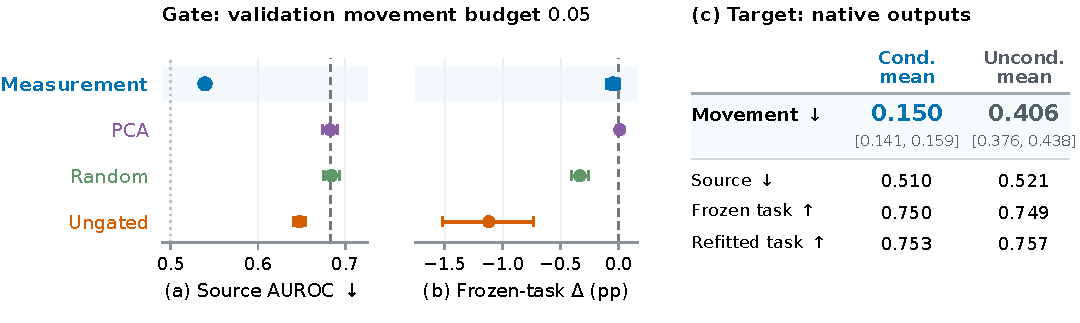
\includegraphics[width=\linewidth]{assets/controlled_mechanisms_compact.pdf}
\caption{\textbf{Where correction acts and what it targets.}
\emph{(a--b) Gate:} source AUROC and paired frozen-task change from identity at a common
$.05$ validation movement budget; dashed lines mark identity and the dotted
line marks chance. Random averages five orientations.
\emph{(c) Target:} conditional versus empirical unconditional mean-score
anchoring, with native 48-stage movement and source/task AUROC.
Three fits, 81 participants; whiskers and movement brackets give 95\%
participant-bootstrap intervals. Budget-matched gates and native target endpoints are separate comparisons.}
\label{fig:gate}
\label{fig:target-cost}
\end{figure}

Measurement-gated correction suppresses source more strongly than all
three controls (Figure~\ref{fig:gate}a). Its frozen-task change from identity is
$-.0005$ $[-.0010,.0001]$, and its advantage over ungated correction is
$.0107$ $[.0069,.0147]$. Attained evaluation movements span $.0504$--$.0539$.
The result distinguishes measurement-supported directions from a generic
restriction of rank or movement. Appendix~\ref{app:gate-attribution}
details the comparison.

\paragraph{Conditioning reduces correction cost.}
\label{sec:ablations}
Conditional-mean anchoring uses $M=.1500$ rather than $.4063$ for the
empirical unconditional mean-score target, which requires about 2.7 times
as much movement (Figure~\ref{fig:target-cost}c). Source AUROC is lower
($.5105$ versus $.5214$), with no clear frozen-task difference; refitted-task
AUROC favors the unconditional target ($.7574$ versus $.7527$).
This links the cost argument in Section~\ref{sec:targets} to learned
correction. Unlike the fixed-score analysis, these trajectories refit their
critics separately. Appendix~\ref{app:target-controls} gives the target
definitions and paired contrasts.

\subsection{Correction on recorded EEG}
\label{sec:real-results}
We next test the construction on two forms of recorded EEG:
240-dimensional temporal N170 features from simultaneous Neuroscan/Flex
recordings \citep{williams2020flex}, and wet/dry SSVEP representations from
frozen EEGPT. Table~\ref{tab:real-main} compares source attenuation and task
utility in both settings.

\paragraph{Temporal N170: nonlinear correction and task utility.}
Genuine calibration pairs support face/watch discrimination. The linear-only
ablation keeps the measurement gate and anchor fixed while removing the
nonlinear critic. At nearly identical movement ($.3449$ versus $.3469$), adding that
critic lowers source accessibility and improves refitted task performance.
Relative to the linear-only ablation, the paired source AUROC change is
$-.0413$ $[-.0647,-.0210]$ and the refitted-task gain is $.0171$
$[.0005,.0384]$. The full correction also
improves both frozen and refitted task AUROC over identity
(Table~\ref{tab:real-main}A; paired intervals in
Appendix~\ref{app:retained-results}).

Direct comparison with IGBP~\citep{iskander2023} tests whether this benefit
extends beyond our own critic ablation. Iterative MGPA improves native
refitted-task AUROC over IGBP by $.0361$
$[.0306,.0405]$ with less movement ($.3469$ versus $.4973$).
At a common $.25$ validation movement budget, it also achieves lower source
AUROC and higher frozen/refitted task AUROC
(Appendix~\ref{app:igbp-comparison}). FEATMAP toward Neuroscan attains
stronger attenuation and higher task scores using source-aware routing
at a larger displacement.

\paragraph{Recorded SSVEP: frozen-model representations.}
\label{sec:recorded-result}
Actual wet/dry sessions test acquisition variation without constructed
embedding interpolation. Because these sessions are not physiological
trial pairs, calibration uses six FIT-local spectral and spatial
transformations of individual trials. Both MGPA constructions correct the
512-dimensional token mean and add the same displacement to all tokens.
Independent source readers and the twelve-frequency task access the
complete $15\times512$ EEGPT representation.

\begin{table}[htbp]
\centering\small
\caption{\textbf{Source attenuation and task utility on recorded EEG.}
Native outputs: N170 (A, 10 participants) and wet/dry SSVEP (B, 21).
$S$: maximum independent source AUROC over the eleven-reader bank in A and
the 41-reader full-input bank in B; $T_f/T_r$: frozen/refitted task AUROC;
$M$: relative movement. Iterative estimates average three fits;
native movements differ. IGBP uses 100 projections with the same
longer-training preset in both studies (Appendix~\ref{app:igbp-protocol}).
Source-aware rows require device identity.
Reference 0/1 denotes Neuroscan/Flex in A and dry/wet in B.
N/A: paired FEATMAP requires physiological wet/dry
trial pairs, unavailable in B.}
\label{tab:real-main}
% Generated by build_experiment_assets.py; see experiment_provenance.json.
\begingroup\small\setlength{\tabcolsep}{3pt}
\begin{tabular*}{\textwidth}{@{\extracolsep{\fill}}llrrrrrrrr@{}}
\toprule
 & & \multicolumn{4}{c}{A. Temporal N170} & \multicolumn{4}{c}{B. Recorded SSVEP} \\
\cmidrule(lr){3-6}\cmidrule(lr){7-10}
Interface & Method & $S\downarrow$ & $T_f\uparrow$ & $T_r\uparrow$ & $M$ & $S\downarrow$ & $T_f\uparrow$ & $T_r\uparrow$ & $M$ \\
\midrule
\multirow{6}{*}{\shortstack[l]{\emph{Source-blind}\\\emph{correction}}} & Identity & 0.989 & 0.728 & 0.728 & 0.000 & 0.916 & 0.688 & 0.688 & 0.000 \\
 & LEACE & 0.980 & 0.728 & 0.727 & 0.234 & 0.918 & 0.689 & 0.689 & 0.102 \\
 & \textbf{MGPA-CF} & 0.982 & 0.727 & 0.728 & 0.237 & 0.895 & 0.689 & 0.690 & 0.056 \\
 & \textbf{MGPA-Iter} & 0.946 & 0.735 & 0.746 & 0.347 & 0.872 & 0.688 & 0.689 & 0.149 \\
 & \quad Linear-only ablation & 0.987 & 0.725 & 0.729 & 0.345 & 0.872 & 0.689 & 0.689 & 0.069 \\
 & IGBP & 0.955 & 0.722 & 0.710 & 0.497 & 0.872 & 0.689 & 0.688 & 0.096 \\
\midrule
\multirow{4}{*}{\shortstack[l]{\emph{Source-aware}\\\emph{alignment}}} & CORAL $\to$ ref. 0 & 0.948 & 0.738 & 0.735 & 0.448 & 1.000 & 0.691 & 0.688 & 0.149 \\
 & CORAL $\to$ ref. 1 & 0.958 & 0.726 & 0.740 & 0.292 & 1.000 & 0.685 & 0.688 & 0.155 \\
 & FEATMAP $\to$ ref. 0 & 0.880 & 0.777 & 0.749 & 0.800 & N/A & N/A & N/A & N/A \\
 & FEATMAP $\to$ ref. 1 & 0.890 & 0.693 & 0.711 & 0.576 & N/A & N/A & N/A & N/A \\
\bottomrule
\end{tabular*}\endgroup

\end{table}

Both constructions reduce full-input source accessibility relative to
LEACE (Table~\ref{tab:real-main}B). The paired source differences for
Closed-form and Iterative MGPA
are $-.0231$ $[-.0459,-.0058]$ and $-.0463$ $[-.0671,-.0225]$.
Frozen/refitted task scores remain close to identity for both constructions.
Thus attenuation extends to the full downstream input, with little observed
change in task utility. IGBP reaches the same full-input source score
($S=.872$) with close task AUROCs and less movement ($.096$ versus $.149$).
Appendix~\ref{app:recorded-full-input} details this
shared-interface comparison. Appendix~\ref{app:full-token-readers} specifies
the full-input audit, and Appendix~\ref{app:retained-results} reports paired
task and component comparisons.

\subsection{Selecting on P300, reusing on N170 and MMN}
\label{sec:recovery}
The preceding studies assess what remains accessible in corrected
representations. We now ask whether one correction can improve the behavior
of predictors for other tasks. Simultaneous Neuroscan/Flex recordings of
P300, N170 and MMN share a fixed EEGPT/PCA representation. We fit and select
each adapter on P300, then apply the same map to N170 and MMN without
target-task adapter tuning. The encoder and task heads remain frozen, so the
comparison tests whether the reused correction improves existing predictions
rather than enabling a newly trained predictor.

For each task, a head trained with device--label association is evaluated
as that association weakens or reverses. Association is changed by selecting
the observed device from real event pairs, without altering the EEG signal.
An independently trained control head measures utility without the induced
association. P300 development data select correction strength under a
worst-association objective and task-utility guardrails, with the same
selection criterion for competitors. Appendix~\ref{app:recovery-protocol}
specifies the fitting and selection protocol.

\begin{table}[htbp]
\centering\small
\caption{\textbf{One P300-selected correction, three frozen task heads.}
Eight common participants; worst-association AUROC of shortcut-trained
heads and independent-regime AUROC of separate control heads. Iterative
scores average three fits, each with an unchanged P300-selected map.
For each fit, worst is the minimum participant-mean AUROC
over association strength. Paired intervals and per-fit results are in
Appendix~\ref{app:transfer-results}.}
\label{tab:reuse-main}
% Generated by build_experiment_assets.py; see experiment_provenance.json.
\begingroup\small\setlength{\tabcolsep}{4pt}
\begin{tabular*}{\textwidth}{@{\extracolsep{\fill}}llrrrrrr@{}}
\toprule
 & & \multicolumn{3}{c}{Worst-association AUROC $\uparrow$} & \multicolumn{3}{c}{Control-head AUROC $\uparrow$} \\
\cmidrule(lr){3-5}\cmidrule(lr){6-8}
Interface & Method & P300 & N170 & MMN & P300 & N170 & MMN \\
\midrule
\multirow{4}{*}{\shortstack[l]{\emph{Source-blind}\\\emph{correction}}} & Identity & 0.355 & 0.122 & 0.446 & 0.627 & 0.622 & 0.640 \\
 & LEACE & 0.601 & 0.384 & 0.614 & 0.622 & 0.621 & 0.639 \\
 & \textbf{MGPA-CF} & 0.599 & 0.420 & 0.642 & 0.627 & 0.621 & 0.642 \\
 & \textbf{MGPA-Iter} & 0.599 & 0.441 & 0.632 & 0.627 & 0.621 & 0.641 \\
\midrule
\multirow{2}{*}{\shortstack[l]{\emph{Source-aware}\\\emph{alignment}}} & CORAL & 0.550 & 0.277 & 0.624 & 0.627 & 0.622 & 0.641 \\
 & FEATMAP & 0.573 & 0.471 & 0.618 & 0.627 & 0.611 & 0.625 \\
\bottomrule
\end{tabular*}\endgroup

\end{table}

\begin{figure}[htbp]
\centering
% Temporary dot-plot alternative; original curves remain in reuse_associations.pdf.
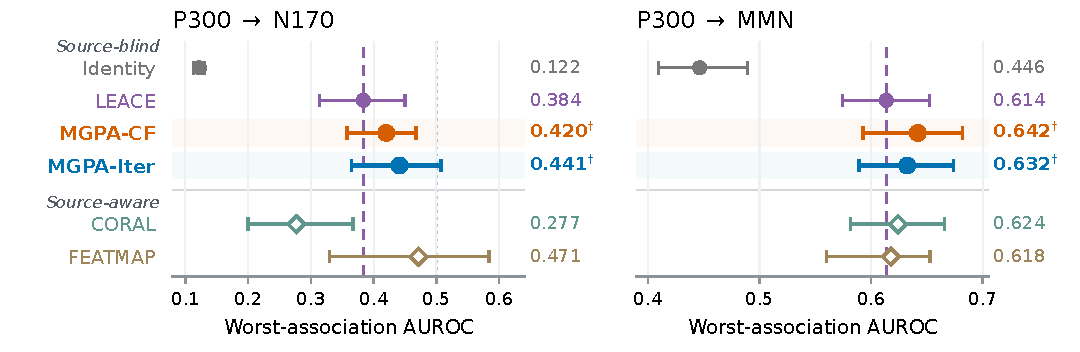
\includegraphics[width=\linewidth]{assets/reuse_worst_preview.pdf}
\caption{\textbf{Reusing a P300-selected correction.}
Absolute worst-association AUROC of frozen N170/MMN shortcut-trained heads;
whiskers show marginal 95\% participant-bootstrap intervals.
Dashed: LEACE; dotted: chance; hollow: source-aware methods.
$\dagger$: paired 95\% interval for the gain over LEACE entirely above zero.
Intervals condition on fitted maps and are unadjusted for multiplicity;
panel ranges differ.}
\label{fig:reuse}
\end{figure}

Both MGPA constructions improve worst-association AUROC over LEACE on
the two transfer tasks (Table~\ref{tab:reuse-main}). Iterative MGPA gains
$.0574$ $[.0338,.0831]$ on N170 and $.0188$ $[.0040,.0241]$ on MMN;
Closed-form MGPA gains $.0364$ $[.0049,.0667]$ and $.0282$ $[.0021,.0343]$,
respectively. Control-head AUROC stays close to identity across all three
tasks. FEATMAP has the highest N170 worst-association score, with lower
N170 and MMN control-head scores; the grouped comparison retains its
source-aware deployment interface.

Figure~\ref{fig:reuse} compares absolute worst-association performance on
both transfer tasks, with LEACE as a reference.
Together, the experiments connect selective correction of representations
to reusable changes in downstream prediction.

% ===== 07_discussion.tex =====
\section{Discussion and Conclusion}
\label{sec:discussion}
MGPA provides a practical way to correct acquisition-sensitive variation in
frozen representations without treating all source-predictive variation as
disposable. Calibration specifies
where edits are supported; it does not imply that everything within that
space should be removed. The correction target must also account for what
is preserved: editable coordinates should not be forced to compensate for
source information that remains available in the fixed complement.

This perspective opens a practical route to adapting pretrained
representations without rebuilding the encoder for each downstream task.
The value of a reusable correction lies not only in changing what a
probe can read, but in changing how an existing predictor behaves when
acquisition cues cease to be reliable.
Closed-form and Iterative MGPA provide two implementations of this principle.
Although evaluated here on EEG, the construction is not EEG-specific: it
requires credible calibration views of the same observation under different
measurement conditions. Richer
calibration could reveal which edit directions remain supported across
acquisition conditions, and which depend on a particular contrast. The
opportunity is to make representation correction more selective and its
assumptions more explicit: \emph{measurement evidence determines where
correction may act, and preserved information shapes what it should aim for.}
\FloatBarrier
\label{sec:main-end}
% ===== statements.tex =====
\section*{Reproducibility Statement}
The supplement provides proofs, calibration and update specifications,
participant roles, selection rules and statistical evaluation details.
Code, configurations and participant-level results are indexed by the
repository README (Appendix~\ref{app:reproduction}), which distinguishes
saved-result reconstruction from fresh experiments.

\section*{Ethics Statement}
This study uses existing research EEG datasets and introduces no new data
collection or clinical intervention. Provenance attenuation does not confer
anonymity or establish clinical validity. Applications involving patients
require task-specific validation and appropriate data governance.

\section*{AI Usage Statement}
Generative artificial intelligence (AI) tools assisted code cleaning,
preliminary literature review and manuscript polishing. The authors retain
responsibility for the final content.
\bibliography{references}
\bibliographystyle{iclr2027/iclr2027_conference}
\clearpage
\appendix
% ===== appendix_proofs.tex =====
\section{Proofs and Solver Details}
\label{app:proofs}
All statements in this section condition on the fitted gate and treat its
orthonormal basis $B$ as fixed. Fixed-score statements also condition on the
critic and correction metric. Norms without a subscript are Euclidean;
$\|v\|_\Omega^2=v^\top\Omega v$.

\subsection{Fixed-complement preservation and the source floor}
\label{app:fixed-complement}
Since $(I-P)B=0$, every admissible correction satisfies
\[
 (I-P)R(h)=(I-P)h=q(h).
\]
Thus $Q$ is recoverable from the corrected representation, and the chain
rule gives \eqref{eq:floor}. Preservation also holds under composition and
fractional steps. For $R_\mu(h)=q(h)+B\mu(q(h))$, the output is determined
by $Q$, so the conditional-information term is zero.

\subsection{Fixed-score geometry and retained information}
\label{app:affine-levels}
\label{app:euclidean-anchor}
In Proposition~\ref{prop:parallel-levels}, the functions $b(q),w(q)$ and
$\Omega(q)\succ0$ are measurable in $q$, with $w(q)\ne0$ almost surely.
The score has finite conditional second moments when costs are evaluated.
For fixed $(q,z)$, matching anchor $a(q)$ requires
$w^\top\Delta=a(q)-s(q,z)$. Metric Cauchy--Schwarz gives
\[
 (a-s)^2\le(w^\top\Omega^{-1}w)\,\Delta^\top\Omega\Delta.
\]
The unique minimizer is $\Delta=v(a-s)$, where
$v=\Omega^{-1}w/d_\Omega$. Its squared norm is $(a-s)^2/d_\Omega$.
The output editable block is
\[
 Z'=N+v\{a(Q)-b(Q)\},\qquad N=(I-vw^\top)Z.
\]
The output is a measurable function of $(Q,N)$; conversely,
$N=Z'-v\{a(Q)-b(Q)\}$ is measurable in the output because $Q$ is
retained. Thus $\sigma(T_a)=\sigma(Q,N)$. Every anchor retains the same
information about $U$ and about any task variable $Y$, including the same
unrestricted Bayes prediction risk. Conditional independence from $U$
holds exactly when $N\perp U\mid Q$. The conditional bias--variance
decomposition of $\E[(s-a)^2\mid Q=q]$ proves
\eqref{eq:affine-cost} and the unique mean-anchor optimum.

For $\Omega=I$, the edit is $w(a-s)/\|w\|^2$ and the denominator is
$\|w\|^2$. Orthonormality of $B$ makes this the Euclidean movement in
the standardized representation as well. The result compares exact
score-level corrections with the same fixed score and metric. Nonlinear
sample-dependent Jacobians, active radius constraints and independently
refitted compositions are not members of that comparison.

\subsection{Proof of Theorem~\ref{thm:compensation}}
\label{app:gaussian-proof}
Fix $q$ and abbreviate $p=p(q)$, $m=m(q)$ and $\kappa=\kappa(q)$.
Expanding the two Gaussian quadratic log densities gives
\[
 \log\frac{p(z\mid q,1)}{p(z\mid q,0)}
 =\delta^\top S^{-1}(z-m)=\ell(q,z).
\]
Let $L=I-\delta\delta^\top S^{-1}/D$. The repaired editable coordinate is
\[
 Z_\kappa=LZ+\frac{\delta}{D}
                  \{\delta^\top S^{-1}m+\kappa\}.
\]
Since $L\delta=0$, its conditional mean is the same for both sources.
Its conditional covariance is $LSL^\top$ for both. The resulting possibly
singular Gaussian laws are identical, proving conditional independence.
The map preserves $Q$ by construction.

Proposition~\ref{prop:parallel-levels}, applied with $w=S^{-1}\delta$ and
$\Omega=S^{-1}$, gives the unique minimum-norm edit
$\Delta=\delta(\kappa-\ell)/D$, with squared cost $(\kappa-\ell)^2/D$.
Conditional on $Q=q,U=u$, the residual score $\ell$ has mean
$(2u-1)D/2$ and variance $D$. Consequently,
\[
 \E[\ell\mid q]=(2p-1)D/2,\qquad
 \Var(\ell\mid q)=D+D^2p(1-p).
\]
Thus
\[
 C_\kappa(q)=\frac{\E[(\ell-\kappa)^2\mid q]}{D}
 =1+Dp(1-p)+\frac{\{\kappa-(2p-1)D/2\}^2}{D},
\]
which is \eqref{eq:gauge-cost}. Its minimum occurs at
$\kappa_*=(2p-1)D/2$. Subtracting this minimum from the cost at
$\kappa=-\sg$ yields \eqref{eq:compensation}. Since $\sg=\logit p$ and
$2p-1$ have the same sign, the excess is strictly positive for $p\ne1/2$.
At fixed such $p$, its numerator tends to $\sg^2>0$ as $D\downarrow0$,
so the excess diverges.

\subsection{Selective mean anchoring and full completion}
\label{app:completion}
The unique minimizer of \eqref{eq:gauge-cost} is
$\kappa_*=(2p-1)D/2$. To show its optimality among deterministic conditional
erasers affine in $Z$, whiten at fixed $q$:
\[
 X=S^{-1/2}(Z-m),\quad v=S^{-1/2}\delta,\quad
 X\mid U=u\sim\mathcal N((2u-1)v/2,I),\quad\|v\|^2=D.
\]
An affine map $X'=FX+c$ erases source exactly if and only if $Fv=0$:
the two output means must coincide, and their covariance already agrees.
For fixed $F$, the least-distortion intercept is $c=(I-F)\E X$. Since
$\Cov(X)=I+p(1-p)vv^\top$, its cost under the erasure constraint is
\[
 \tr\{(F-I)\Cov(X)(F-I)^\top\}
 =\|F-I\|_F^2+p(1-p)D,\qquad Fv=0.
\]
The unique matrix nearest $I$ in Frobenius norm subject to $Fv=0$ is
$F_*=I-vv^\top/D$. Unwhitening gives precisely $R_{\kappa_*}$, with
cost $1+Dp(1-p)$. This is the conditional binary affine-erasure geometry
of LEACE \citep{belrose2023}.

For quotient-only completion, the best fixed-$q$ choice is
$Z'=\E[Z\mid q]$. Its cost is the $S^{-1}$ trace of
$\Cov(Z\mid q)=S+p(1-p)\delta\delta^\top$, hence
$r+Dp(1-p)$, exceeding the selective correction cost by $r-1$.

\subsection{Proof of Corollary~\ref{cor:direction-error}}
\label{app:direction-error}
Fix the fitted quantities and $q$. The editable part of $T_a$ is
$Z'=MZ+v\{a(q)-b(q)\}$, where
\[
 M=I-\frac{\widehat\delta\widehat\delta^\top C^{-1}}
 {\widehat\delta^\top C^{-1}\widehat\delta},
 \qquad \ker M=\operatorname{span}(\widehat\delta).
\]
The translation is shared by both sources. Their output mean difference is
$M\delta$ and their common covariance is $MSM^\top$. With $+$ denoting
the Moore--Penrose inverse, put $A=MS^{1/2}$ and $x=S^{-1/2}\delta$.
An SVD shows that $A^\top(AA^\top)^+A$ is the orthogonal projector onto
$(\ker A)^\perp$. Since
$\ker A=\operatorname{span}(S^{-1/2}\widehat\delta)$,
\[
 D_{\rm out}=(M\delta)^\top(MSM^\top)^+(M\delta)
 =x^\top A^\top(AA^\top)^+Ax
 =D-\frac{(\delta^\top S^{-1}\widehat\delta)^2}
 {\widehat\delta^\top S^{-1}\widehat\delta}.
\]
Dividing by $D>0$ proves \eqref{eq:direction-residual}. No equality between
the fitted $C$ and evaluation covariance $S$ is needed. The latter defines
the angle and separation; it need not be available to the algorithm.

This is a conditional identity for any fitted direction, not a bound on its
estimation error. Such a bound requires a calibration model relating the
paired contrasts to the conditional shift $\delta$; the learned gate alone
does not supply it. The full-step qualification is essential: for
$M_\alpha=I-\alpha(I-M)$, $\det M_\alpha=1-\alpha$. Thus for
$\alpha\ne1$ the map is invertible given $Q$ and preserves the exact
conditional source information and covariance-adjusted separation, even
though a fixed prediction head can respond differently.

\subsection{Estimating the same conditional-mean anchor}
\label{app:anchor-estimation}
Fix the gate, affine score, metric and evaluation distribution in
Proposition~\ref{prop:parallel-levels}. Let an anchor-fitting sample
$\mathcal C$, independent of the evaluation observation, produce a
$Q$-dependent anchor $\widehat a_{\mathcal C}(q)$ with finite mean-squared error.
Writing $\mu(q)=\E[s\mid Q=q]$, Proposition~\ref{prop:parallel-levels}
and expectation over $\mathcal C$ give
\begin{equation}
 \E_{\mathcal C}\mathcal C_{\widehat a_{\mathcal C}}(q)-\mathcal C_\mu(q)
 =\frac{\E_{\mathcal C}\{\widehat a_{\mathcal C}(q)-\mu(q)\}^2}{d_\Omega(q)}.
 \label{eq:anchor-risk}
\end{equation}
Thus the estimated anchor has lower expected squared movement than a fixed
reference $a_0(q)$ exactly when its estimation mean-squared error is below
$\{a_0(q)-\mu(q)\}^2$. This is an out-of-sample comparison conditional
on the fixed score and gate.

\subsection{The smooth trust-region step}
\label{app:solver}
For the editable Jacobian $A$ and critic residual vector $e$ in
Section~\ref{sec:method}, smooth weighting balances the gated gradient scales:
\begin{equation}
 W_{jj}=(\|A_j\|^2+\lambda^2)^{-1/2},\qquad
 \bar A=WA,\quad\bar e=We,\qquad\lambda>0.
 \label{eq:normalization}
\end{equation}
For $\lambda,\tau,\rho>0$, the objective in \eqref{eq:tr-problem} is
strictly convex on a compact convex ball. Its unique minimizer has the
standard trust-region form \citep{more1983}
\begin{equation}
 \Delta z_*=-\bar A^\top\{\bar A\bar A^\top+(\tau+\nu)I\}^{-1}\bar e,
 \quad\nu\ge0,\quad\nu(\|\Delta z_*\|-\rho)=0.
 \label{eq:tr-solution}
\end{equation}
The stationarity condition
\[
 (\bar A^\top\bar A+(\tau+\nu)I)\Delta z_*=-\bar A^\top\bar e
\]
yields the stated $J\times J$ solution. Set $\nu=0$ when the unconstrained
step is feasible; otherwise its norm decreases continuously with $\nu$,
and a scalar solve enforces $\|\Delta z_*\|=\rho$. Since $B$ is orthonormal,
the radius directly bounds the embedding edit:
$\|h^+-h\|=\|\Delta z_*\|\le\rho$.
% ===== appendix_protocol.tex =====
\section{Experimental Protocols}
\label{app:protocols}
\label{app:protocol}
FIT determines coordinates, gates and adapters; VAL sets prescribed movement
endpoints; HEAD trains independent readers; EVAL supplies participant scores.
Participant roles are disjoint within a split. Table~\ref{tab:protocol-map}
distinguishes native outputs, matched movement and task-informed P300 DEV
selection. Downstream labels construct associations and train heads, but
enter adapter selection only in reuse and never adapter fitting.
The repository README (Appendix~\ref{app:reproduction}) indexes participant
lists, executable configurations and per-study reproduction instructions.

\begin{table}[htbp]
\centering\small
\caption{\textbf{Protocol map.} Participant counts are FIT/VAL/HEAD/EVAL
(DEV replaces VAL in reuse). Gates are fixed during correction.}
\label{tab:protocol-map}
\begin{tabular}{@{}>{\raggedright\arraybackslash}p{.18\linewidth}>{\raggedright\arraybackslash}p{.43\linewidth}>{\raggedright\arraybackslash}p{.33\linewidth}@{}}
\toprule
Study & Coordinates, calibration and gate & Participants and operating point \\
\midrule
Controlled SSVEP & Pooled EEGPT512; full same-trial CAR/Oz contrasts;
90\% directional energy, ranks $3,3,3,2$ & Four role rotations;
81 distinct EVAL participants. Native correction/target; $.05$ VAL budget for permission. \\
\addlinespace
Temporal N170 & 240 temporal features; simultaneous Neuroscan/Flex pairs;
90\% energy, rank 56 & $4/2/4/10$; native maps and matched-budget IGBP comparison. \\
\addlinespace
Recorded SSVEP & Mean512 correction, $15\times512$ readouts;
six virtual FIT-local contrasts; 99\% energy, rank 328 & $41/20/20/21$;
native maps. \\
\addlinespace
P300-selected reuse & EEGPT/PCA256, P300 FIT reference coordinates;
400 simultaneous CAL pairs, rank 8 & $4/2/4/8$;
P300 DEV-selected map, unchanged on N170/MMN. \\
\bottomrule
\end{tabular}
\end{table}

\subsection{Measurement views and participant roles}
\paragraph{Controlled SSVEP.}
The wet/dry collection contains 102 participants, 12 frequencies and ten
blocks per frequency and electrode type \citep{zhu2021ssvep}. Wet trials
from eight occipital channels are cropped to samples 160--659 at 250 Hz,
standardized within channel and encoded by frozen EEGPT
\citep{wang2024eegpt}. CAR and Oz-reference views are encoded separately;
averaging 15 tokens yields $h_i^{\rm CAR},h_i^{\rm Oz}\in\R^{512}$.
The evaluated endpoints are
\[
 h_i(u)=\tfrac12(h_i^{\rm CAR}+h_i^{\rm Oz})
 +(2u-1)\tfrac{\gamma}{2}(h_i^{\rm Oz}-h_i^{\rm CAR}),\qquad\gamma=.005,
\]
whereas calibration uses the full CAR--Oz contrasts. The task is frequency
$\geq12$ Hz. Within each FIT/VAL participant--frequency cell, nine of ten
trials receive source 1 in the high-frequency class and one of ten in the
low-frequency class. Adapters fit these observed endpoints; HEAD/EVAL
readers use both endpoints with equal source mass.

Five folds are stratified by electrode-session order and gender. In rotation
$r$, folds $r,r+1,r+2$ supply EVAL, HEAD, VAL cyclically, and the remaining
two supply FIT. The four FIT/VAL/HEAD/EVAL counts are $41/20/20/21$,
$42/20/20/20$, $41/21/20/20$ and $40/21/21/20$. Each participant supplies
120 underlying trials. The 81 distinct EVAL participants appear once per
fit seed; source assignment is fixed across seeds. Closed-form comparisons
use one deterministic map per split and the seed-17 reader realization;
gate/target comparisons cross these rotations with all shared fit seeds.

\paragraph{Temporal N170.}
Neuroscan (source 0) and Flex (source 1) record the same watch/face events
concurrently \citep{williams2020flex}. Processing uses 16 common channels,
0.1--30 Hz zero-phase FIR filtering, CAR, resampling to 128 Hz, and one-second
epochs starting at $-.2$ s with prestimulus baseline subtraction. Event
ordinals and timestamps align the views. A pair is retained only if neither
device exceeds $100\,\mu$V absolute amplitude after baseline correction.
FIT/VAL/HEAD/EVAL contain $622/288/716/1381$ clean pairs; every EVAL
participant retains both classes. Fifteen successive 50 ms channel averages
from 0 to 750 ms give 240 coordinates without an encoder or PCA. This is
distinct from the EEGPT-based reuse protocol below.

\paragraph{Recorded SSVEP.}
Source 0/1 denotes actual dry/wet sessions, with no physiological trial
correspondence. The roles contain $9840/4800/4800/5040$ observations under
one fixed stratified split. Six calibration transformations of each trial
use spectral transport, spatial transport and their composition at strengths
.5 and 1 toward the opposite source. FIT prestimulus signals determine
smoothed log-power gains clipped to $[.25,4]$ and spatial whitening/coloring
with covariance shrinkage .1. MGPA corrects the token mean and adds its
displacement to every token; source and twelve-frequency task readers
access the full $15\times512$ representation.

\subsection{Fitting, replay and comparison interfaces}
\label{app:fitting-replay}
\label{app:component-fitting}
\begin{table}[htbp]
\centering\small
\caption{\textbf{Shared MGPA settings.} Component ablations change only the
specified critic or target. Split, reader and assignment seeds are separate.}
\label{tab:shared-settings}
\begin{tabular}{@{}>{\raggedright\arraybackslash}p{.34\linewidth}>{\raggedright\arraybackslash}p{.60\linewidth}@{}}
\toprule
Component & Setting \\
\midrule
Iterative fits / horizon & Seeds 17, 29, 43; at most 48 stages \\
Source critics & Balanced logistic ($C=1$); GELU MLP, hidden width 128 \\
Conditional-mean anchor & Ridge with intercept and penalty 10 (both constructions) \\
Neural-critic optimizer & AdamW, batch 256, weight decay $.001$ \\
Gradient stabilizer / damping & $.1$ / $.001$ \\
Controlled and real-representation fits & 12 critic epochs, LR $.001$, radius $.05\sqrt d$ \\
P300 reuse fits & At most 100 epochs, LR $.0003$, source-VAL patience 10,
radius $.025\sqrt d$ \\
Closed-form residual covariance & $.01$ shrinkage toward mean-diagonal identity \\
Participant uncertainty & 20,000 percentile bootstrap resamples, seed 1101 \\
\bottomrule
\end{tabular}
\end{table}

\begin{algorithm}[htbp]
\small
\caption{Iterative MGPA: fit once, replay without source labels}
\label{fig:algorithm-main}
\begin{enumerate}
\setlength{\itemsep}{2pt}
\item \textbf{Inputs:} calibration pairs, source-labeled FIT/VAL embeddings,
gate rank or energy threshold, critic bank, $\lambda,\tau,\rho,K$, and
endpoint rule. Task-informed selection additionally requires DEV task data.
\item Fit standardization and the contrast-SVD gate \eqref{eq:gate-estimate};
freeze $B,P,Q$. Return identity if $r=0$. Store original FIT/VAL complements.
\item Fit source critics on current FIT embeddings and regress their scores
on original FIT $Q$ to obtain conditional anchors.
\item Store critics and anchors; compute $e,A,W$, solve
\eqref{eq:tr-problem}, and apply $h\leftarrow h+B\Delta z_*$. Record VAL
outputs and repeat Steps 3--4 up to $K$ stages.
\item Select and store the prefix and optional final-stage fraction using
the declared validation rule; only task-informed selection uses task labels.
\item \textbf{Deployment:} standardize one embedding, replay the stored map,
and return it in the downstream interface's coordinates.
\end{enumerate}
\end{algorithm}

Standardization uses FIT only. Gates use row-normalized contrasts;
controlled and N170 fits filter contrast norms at the fifth percentile,
whereas recorded SSVEP uses no percentile filter. Controlled gating uses
at most 2048 deterministically sampled contrasts. Energy thresholds and
ranks appear in Table~\ref{tab:protocol-map}.
Closed-form MGPA uses the same gate and standardization, the mean projected
calibration contrast, and the shared Ridge anchor. Its metric comes from
residuals of a joint regression of $Z$ on $Q$ and source: intercept/source
coefficients are unpenalized and $Q$ has penalty 10. The residual second
moment is normalized by FIT count and shrunk as in
Table~\ref{tab:shared-settings}; \eqref{eq:closed-form-mgpa} uses linear
solves. Native studies take $\alpha=1$; reuse selects $\alpha$ on DEV.
Recorded contrasts are oriented wet-like to dry-like for both gate and direction.

The target ablation replaces the conditional anchor by the current-stage
empirical FIT-mean score; a zero-score control is also reported. The
linear-only ablation removes the nonlinear critic. Other fitting settings
remain matched as specified in the corresponding results.

\paragraph{Baselines and deployment information.}
LEACE fits an unrestricted covariance-weighted affine eraser to observed
FIT rows. CORAL uses FIT source means and identity-regularized sample
covariances, not pair correspondence. FEATMAP fits centered unregularized
least squares to FIT pairs, with the minimum-norm slope for rank-deficient
designs; controlled pairs use the evaluated $\gamma$-scaled endpoints.
CORAL/FEATMAP leave their chosen reference unchanged and require source
routing at deployment; both orientations are reported. MGPA, LEACE and
IGBP deploy source-blind. Recorded SSVEP has no paired FEATMAP comparison.
No method uses EVAL moments. Reuse searches regularization/strength on
P300 DEV instead of using these native settings.

\paragraph{IGBP.}
\label{app:igbp-protocol}
IGBP~\citep{iskander2023} shares each study's roles, standardized inputs and
independent readers. At each iteration a $d\to d\to2$ ReLU classifier
drives an ungated projective update without a conditional anchor or pair
correspondence. All reported fits use the longer-training preset: AdamW,
LR $2\times10^{-4}$, weight decay $.01$, batch 256, at most 50 epochs,
VAL source-accuracy patience 10 and improvement threshold $.002$, with no
$.80$ accuracy exit. Native maps apply 100 projections without task-based
stopping. Updates are evaluated directly in logit space to avoid softmax
saturation. For N170, $d=240$; for recorded SSVEP, $d=512$ and the resulting
mean correction is added to every token, matching MGPA's interface.

\paragraph{Matched movement and edit-permission controls.}
\label{app:gate-attribution}
Native outputs apply the complete fitted map; movements need not match.
A budget $b$ instead selects the first
upward crossing of $\|H'_{\rm VAL}-H_{\rm VAL}\|_F/\|H_{\rm VAL}\|_F=b$,
interpolating only the last update and replaying that prefix/fraction on
HEAD/EVAL. Controlled permission compares the measurement gate, leading
observed-FIT PCA directions of the same rank, five fixed random orientations
of that rank (averaged, not selected), and all 512 directions. Each arm
refits its critics and anchors with the same recipe and original measurement
complement $Q_0$ as anchor input. Thus controls receive calibration-derived
rank and conditioning information; only the measurement arm necessarily
preserves $Q_0$. Every correction arm and random orientation attains the
reported $.05$ budget; all 108 cells, including identity, are available.
At the originally primary $.10$ budget, 17 of 60 random trajectories
do not attain it within the horizon; native endpoints are not substituted.
The N170 IGBP budget comparison uses the same first-crossing rule.

\subsection{Independent readers and statistical summaries}
\label{app:independent-readouts}
\label{app:full-token-readers}
Source readers fit corrected HEAD outputs independently of adapters and
score participant-disjoint EVAL outputs. Table~\ref{tab:reader-bank} specifies
their inputs and capacity. All preprocessing uses HEAD only; each recording,
not each token, is one example. Neural readers train without early stopping
and contribute three restarts at 12/50/200 epochs.

\begin{table}[htbp]
\centering\small
\caption{\textbf{Independent source-reader bank.} Controlled/N170 use the
11 common readers. Recorded SSVEP uses all $11+20+10=41$ readers; its common
bank alone defines $S_{\rm mean}$.}
\label{tab:reader-bank}
\begin{tabular}{@{}>{\raggedright\arraybackslash}p{.23\linewidth}>{\raggedright\arraybackslash}p{.71\linewidth}@{}}
\toprule
Input & Readers and training \\
\midrule
Common representation & Ordinary and covariance-whitened logistic ($C=1$,
whitening shrinkage $.01$); GELU MLP with width 128, AdamW, LR $.001$,
batch 256, weight decay $.001$. \\
\addlinespace
Direct full tokens & Raw logistic ($C=1$), HEAD-standardized logistic
($C=.01$); flat $7680\to128\to2$ GELU with common training; token network
with LayerNorm, shared $512\to64$ GELU, concatenation and binary output,
LR $.0005$, batch 128, weight decay $.001$, gradient clipping 5. \\
\addlinespace
Centered token residuals & Standardized logistic and the same token network
with its three restarts/checkpoints. \\
\bottomrule
\end{tabular}
\end{table}

Recorded common-offset correction preserves $R_t=H_t-\bar H$.
Residual readers fit once on original HEAD residuals and are reused on
corrected EVAL; numerical invariance is checked. This retained token
variation is distinct from the pooled gate complement $Q$.

\paragraph{Task utility and movement.}
Controlled/N170 heads are HEAD-standardized balanced Ridge classifiers
(penalty 10, LSQR). The recorded task head uses HEAD-standardized flattened
features and the token architecture above with a twelve-class output,
trained for 50 epochs. Frozen heads and scalers train on original HEAD;
refitted heads and scalers train on corrected HEAD; both evaluate corrected
EVAL. $T_f/T_r$ equally average participant AUROCs over $0\to1$ and
$1\to0$ transfer; recorded scores are twelve-class macro AUROC.
$M$ averages $\|H'_p-H_p\|_F/\|H_p\|_F$ over EVAL participants, which
can differ from aggregate VAL movement.

\paragraph{Aggregation and uncertainty.}
\label{app:evaluation-scope}
Source accessibility maximizes participant-mean AUROC over readers within
each fit, then averages fits. Controlled scores pool disjoint EVAL folds;
deterministic maps contribute one output per split. Shared participant
bootstrap draws pair methods, transfer directions and fits, recomputing
the source maximum inside every draw. Intervals condition on fitted
coordinates, adapters and readers and are pointwise, without multiplicity
adjustment; seeds/trials do not increase participant counts. These cohorts
informed protocol development, including the P300 selection task and rank
eight. Controlled gate/target studies share participants; the two N170
protocols overlap. Source maxima measure accessibility under the specified
bank, not complete erasure or unbiased performance of an EVAL-selected reader.

\subsection{P300-selected correction reused on N170 and MMN}
\label{app:recovery-protocol}
\label{app:reuse-protocol}
\paragraph{Calibration and shared coordinates.}
All three tasks use simultaneous Neuroscan/Flex recordings and the same
eight EVAL participants. The first 100 consecutive P300 pairs per FIT
participant form CAL. Any other FIT event whose one-second epoch overlaps
CAL on either device is excluded, leaving 2260 observed events. One endpoint
per observed event plus both endpoints of the 400 CAL pairs yields 3060
unique fitting endpoints for MGPA, LEACE and CORAL; FEATMAP uses the 400
pairs. CAL supplies both MGPA gates and the Closed-form direction;
Iterative critics fit the pooled bank without paired targets.

Frozen EEGPT retains $7\times4\times512=14{,}336$ features from seven
overlapping windows, with fixed $20\,\mu$V input scaling. Centered PCA256
and standardization fit only the Neuroscan endpoints of remaining P300 FIT
events, then apply to both devices and all tasks. Neither N170 nor MMN
fits coordinates or selects the adapter. HEAD uses all technically valid
events, unlike the amplitude-filtered temporal N170 study.

\paragraph{Frozen heads and association shifts.}
Each task has two balanced logistic heads trained on original HEAD features
with equal participant weights: an aligned, shortcut-sensitive head and an
independent-assignment control head. Regularization is selected from
$C\in\{10^{-6},10^{-5},\ldots,10\}$ by leave-one-HEAD-participant-out
independent-head AUROC and shared between that task's heads. Heads,
standardizers and assignment realizations stay fixed across adapter fits.
For positive-class prevalence $\pi_p$, endpoint assignment satisfies
\[
 \Pr(U=1\mid Y=y,p;\xi)=\tfrac12+.4\xi
 \frac{y-\pi_p}{\max(\pi_p,1-\pi_p)},\qquad \xi\in[-1,1].
\]
Aligned/independent/reversed settings are $\xi=1/0/-1$; device marginals
remain one half and signals are unchanged. Fitting samples recorded
endpoints; evaluation weights both endpoints. Worst AUROC is the exact
minimum of the participant-mean quadratic AUROC curve on $[-1,1]$,
including interior minima. Control-head AUROC is evaluated at $\xi=0$.

\paragraph{Selection and transfer.}
Both MGPA constructions use rank-eight gates and pooled conditional-mean
targets. Iterative training follows Table~\ref{tab:shared-settings}, with
1332 DEV source-validation endpoints. P300 DEV selects the endpoint
maximizing worst AUROC subject to at most $.01$ loss from identity for
\emph{each} head at independent association. Ties prefer less movement,
then an earlier endpoint. All iterative prefixes are eligible. Affine
strengths are $0,.02,\ldots,1,1.1,1.2,1.3$; baseline ridge grids and both
CORAL/FEATMAP reference choices are searched under the same rule. Across
recipes within a family, candidates within $.002$ of the best admissible
DEV worst AUROC are ordered by movement and the fixed tie rule. The grids
and selected values are recorded in the repository's task-reuse guide;
Closed-form MGPA selects $\alpha=1.1$. Each complete selected map is then
reused unchanged on P300, N170 and MMN.

Reuse movement for DEV tie-breaking is the participant mean of the ratio
of mean paired-event displacement norm to mean input norm, rather than the
Frobenius ratio above. Reported worst AUROC averages fit-specific minima
of participant-mean curves, not the minimum of an ensemble curve.
Each shared participant-bootstrap draw recomputes every curve and its
minimum before averaging fits; the same draws pair all tasks and methods.
Control-head AUROCs average participants and fits. Other uncertainty
conventions follow Appendix~\ref{app:evaluation-scope}.

\section{Supporting Experimental Results}
\label{app:retained-results}
Paired intervals follow Appendix~\ref{app:independent-readouts}.

\subsection{Controlled correction and target choice}
\label{app:closed-form-controlled}
\label{app:target-controls}
\paragraph{Closed-form correction.}
In Table~\ref{tab:controlled-cf}, Closed-form MGPA changes source AUROC from
identity by $-.173$ $[-.180,-.164]$. Frozen- and refitted-task changes are
$-.0002$ $[-.0007,+.0002]$ and $+.0004$ $[-.0001,+.0008]$;
the refitted-task gain over LEACE is $+.0879$ $[.0762,.0998]$.

\paragraph{Conditional versus unconditional targets.}
The unconditional control uses each critic's empirical mean score on the
current corrected FIT inputs, recomputed at every stage without downstream
labels or HEAD/EVAL data. Gate, critic fitting, solver and the 48-stage
horizon are unchanged. Each trajectory refits its critics, testing learned
correction rather than the fixed-score equivalence of
Proposition~\ref{prop:parallel-levels}. Zero-score targeting remains a
separate control: balanced source labels do not imply a zero mean logit.

\begin{table}[htbp]
\centering\small
\caption{\textbf{Conditional versus constant targets.}
Native controlled outputs for the same 81 participants and fits as
Figure~\ref{fig:target-cost}c. $S$: source AUROC; $T_f/T_r$: frozen/refitted
task AUROC; $M$: movement.}
\label{tab:target-controls}
% Generated by build_experiment_assets.py; see experiment_provenance.json.
\begingroup\small\setlength{\tabcolsep}{4pt}
\begin{tabular}{@{}lrrrr@{}}
\toprule
Target & $S\downarrow$ & $T_f\uparrow$ & $T_r\uparrow$ & $M$ \\
\midrule
Conditional mean & 0.5105 & 0.7496 & 0.7527 & 0.1500 \\
Unconditional mean (FIT) & 0.5214 & 0.7488 & 0.7574 & 0.4063 \\
Zero score & 0.5199 & 0.7479 & 0.7562 & 0.4172 \\
\bottomrule
\end{tabular}\endgroup

\end{table}

Conditional minus empirical-unconditional anchoring gives movement
$-.2563$ $[-.2907,-.2232]$ and source AUROC $-.0110$ $[-.0143,-.0079]$.
Frozen-task change is $+.0008$ $[-.0015,.0030]$; refitted-task change is
$-.0047$ $[-.0070,-.0025]$.

\subsection{Temporal N170: nonlinear correction and task utility}
\label{app:critic-complexity}
\label{app:igbp-comparison}
\paragraph{Linear-only ablation.}
Removing the GELU critic retains the gate, Ridge mean anchor, smooth
weighting, trust-region radius and stage horizon. Single-critic damping
$.0005$ preserves regularization relative to mean critic loss, equivalently
duplicating the affine constraint at the shared two-critic damping.
Sample-dependent bounded steps make this a linear-critic ablation, not a
globally affine map. Closed-form MGPA instead estimates its direction and
covariance metric from measurement contrasts and the joint residual model.
Table~\ref{tab:critic-complexity} shows why the distinction matters:
linear-only correction lowers linear accessibility but leaves nonlinear
accessibility nearly intact. Iterative MGPA lowers the full-bank score
with higher task scores at nearly the same movement.

\begin{table}[htbp]
\centering\small
\caption{\textbf{Nonlinear critics on N170.} A: strongest linear reader $L$
versus full-bank $S$ for the ten participants in Table~\ref{tab:real-main}A.
B: Iterative minus linear-only AUROC percentage points, with paired 95\%
intervals. Iterative estimates average fits; linear-only is deterministic.}
\label{tab:critic-complexity}
\label{tab:critic-complexity-paired}
% Generated by build_experiment_assets.py; see experiment_provenance.json.
\begingroup\small\setlength{\tabcolsep}{4pt}
\begin{tabular*}{\textwidth}{@{\extracolsep{\fill}}lrr@{}}
\toprule
\multicolumn{3}{@{}l}{\textbf{A. Native source accessibility}} \\
Correction & $L\downarrow$ & $S\downarrow$ \\
\midrule
Identity & 0.763 & 0.989 \\
MGPA-Iter & 0.794 & 0.946 \\
Linear-only & 0.663 & 0.987 \\
\bottomrule
\end{tabular*}\endgroup
\par\vspace{4pt}
% Generated by build_experiment_assets.py; see experiment_provenance.json.
\begingroup\small\setlength{\tabcolsep}{4pt}
\begin{tabular*}{\textwidth}{@{\extracolsep{\fill}}lrrr@{}}
\toprule
\multicolumn{4}{@{}l}{\textbf{B. MGPA-Iter minus Linear-only (AUROC percentage points)}} \\
Contrast & $\Delta S\downarrow$ [95\% CI] & $\Delta T_f\uparrow$ [95\% CI] & $\Delta T_r\uparrow$ [95\% CI] \\
\midrule
Paired difference & -4.13 [-6.47, -2.10] & +0.93 [-0.05, +1.88] & +1.71 [+0.05, +3.84] \\
\bottomrule
\end{tabular*}\endgroup

\end{table}

\paragraph{Comparison with IGBP.}
At native outputs, Iterative MGPA minus IGBP gives frozen/refitted task
gains of $+.0123$ $[.0042,.0203]$ and $+.0361$ $[.0306,.0405]$, and movement
lower by $.1504$ $[.1230,.1769]$. The source-AUROC difference is
$-.0091$ $[-.0198,.0006]$. At common VAL movement budget $.25$
(Table~\ref{tab:igbp-budget}), the respective source, frozen-task and
refitted-task differences are $-.0234$ $[-.0393,-.0099]$,
$+.0082$ $[.0015,.0154]$ and $+.0156$ $[.0063,.0269]$.
At budget $.10$, source accessibility is lower but a downstream advantage
is not established. These comparisons assess complete correction
procedures; equal iteration counts would not equalize their computation.

\begin{table}[htbp]
\centering\small
\caption{\textbf{N170: MGPA versus IGBP at matched VAL budgets.}
First-crossing endpoints follow Appendix~\ref{app:gate-attribution};
attained EVAL movement $M$ may differ. Same ten participants and shared fits.}
\label{tab:igbp-budget}
% Generated by build_experiment_assets.py; see experiment_provenance.json.
\begingroup\small\setlength{\tabcolsep}{4pt}
\begin{tabular}{@{}llrrrr@{}}
\toprule
VAL budget & Method & $S\downarrow$ & $T_f\uparrow$ & $T_r\uparrow$ & $M$ \\
\midrule
.10 & MGPA-Iter & 0.9850 & 0.7274 & 0.7300 & 0.0974 \\
.10 & IGBP & 0.9893 & 0.7292 & 0.7284 & 0.0898 \\
\addlinespace[2pt]
.25 & MGPA-Iter & 0.9643 & 0.7292 & 0.7394 & 0.2422 \\
.25 & IGBP & 0.9877 & 0.7210 & 0.7237 & 0.2239 \\
\bottomrule
\end{tabular}\endgroup

\end{table}

\paragraph{Task utility.}
Iterative MGPA improves frozen/refitted task AUROC over identity by
$+.0070$ $[+.0012,+.0131]$ and $+.0187$ $[+.0042,+.0366]$, respectively.
Both transfer directions receive equal weight:
the refitted gain is concentrated in Neuroscan-to-Flex ($.608$ to $.648$),
while the reverse direction changes from $.847$ to $.844$.

\subsection{Recorded SSVEP: full-input accessibility and utility}
\label{app:recorded-full-input}
On the same saved outputs and participant roles, Iterative MGPA gives
pooled source AUROC $.7954$ and full-bank $S=.8718$, versus identity's
$.9155$. Readers trained directly on all tokens independently support
attenuation: their maximum falls from $.8987$ to $.8685$, a paired change
of $-.0302$ $[-.0459,-.0174]$. The full-bank difference from LEACE is
$-.0463$ $[-.0671,-.0225]$. Closed-form MGPA gives $S=.8949$, a change
of $-.0206$ $[-.0356,-.0043]$ from identity. All maps share the 41-reader bank
(Appendix~\ref{app:full-token-readers}).

Residual-only readers attain $.8718$ for every common-offset correction;
this determines the full-bank maximum for Iterative MGPA, linear-only MGPA
and IGBP. Thus the maximum also reflects retained temporal structure.
CORAL reaches $S=1$ in both orientations under the common-offset interface;
these are not results for token-specific CORAL maps.

\paragraph{Comparison with IGBP and task utility.}
IGBP and Iterative MGPA both attain full-bank $S=.8718$, with pooled-mean
scores $.7832$ and $.7954$, respectively. IGBP has lower movement
($.0956$ versus $.1490$), slightly higher frozen-task AUROC ($.6891$ versus
$.6880$), and similar refitted-task AUROC ($.6884$ versus $.6886$).
Against identity, Iterative MGPA's frozen/refitted task changes are
$-.0002$ $[-.0017,+.0013]$ and $+.0004$ $[-.0028,+.0034]$.

\subsection{P300-selected reuse: absolute outcomes and paired comparisons}
\label{app:transfer-results}
\label{app:reuse-results}
Tables~\ref{tab:reuse-absolute}--\ref{tab:reuse-paired} supplement the main
reuse comparison at its unchanged P300-selected operating points.
Both MGPA corrections improve
transferred worst AUROC over LEACE on N170 and MMN, with paired intervals
excluding zero; on P300 these intervals contain zero. Control-head changes
from identity are small: Closed-form MGPA gains $.0012$ $[.0006,.0018]$ on
MMN, while the other three MGPA transfer-task intervals contain zero.
N170 worst AUROC remains below .5: the gain is improved robustness rather
than complete recovery.

\begin{table}[htbp]
\centering\small
\caption{\textbf{Absolute reuse outcomes.} A/I/R: aligned/independent/reversed
AUROC of the shortcut-sensitive head; worst/control results are in
Table~\ref{tab:reuse-main}. Iterative entries average fits; other maps are
evaluated once. CORAL/FEATMAP require device identity.}
\label{tab:reuse-absolute}
% Generated by build_experiment_assets.py; see reuse_absolute_compact.provenance.json.
\begingroup\small\setlength{\tabcolsep}{4pt}
\begin{tabular*}{\textwidth}{@{\extracolsep{\fill}}lrrrrrrrrr@{}}
\toprule
 & \multicolumn{3}{c}{P300} & \multicolumn{3}{c}{N170} & \multicolumn{3}{c}{MMN} \\
\cmidrule(lr){2-4}\cmidrule(lr){5-7}\cmidrule(lr){8-10}
Method & A & I & R & A & I & R & A & I & R \\
\midrule
Identity & 0.770 & 0.568 & 0.355 & 0.914 & 0.547 & 0.122 & 0.753 & 0.603 & 0.446 \\
LEACE & 0.604 & 0.602 & 0.601 & 0.782 & 0.590 & 0.384 & 0.614 & 0.633 & 0.652 \\
MGPA-CF & 0.643 & 0.621 & 0.599 & 0.735 & 0.579 & 0.420 & 0.642 & 0.644 & 0.646 \\
MGPA-Iter & 0.636 & 0.617 & 0.599 & 0.744 & 0.594 & 0.441 & 0.632 & 0.639 & 0.646 \\
CORAL & 0.662 & 0.607 & 0.550 & 0.818 & 0.564 & 0.277 & 0.639 & 0.632 & 0.624 \\
FEATMAP & 0.625 & 0.600 & 0.573 & 0.697 & 0.591 & 0.471 & 0.623 & 0.621 & 0.618 \\
\bottomrule
\end{tabular*}\endgroup

\end{table}

\begin{table}[htbp]
\centering\small
\caption{\textbf{Paired reuse gains.} Method-minus-comparator AUROC and 95\%
intervals, recomputing worst AUROC inside each bootstrap draw
(Appendix~\ref{app:reuse-protocol}).}
\label{tab:reuse-paired}
% Generated by build_experiment_assets.py; see experiment_provenance.json.
\begingroup\small\setlength{\tabcolsep}{4pt}
\begin{tabular*}{\textwidth}{@{\extracolsep{\fill}}lllrr@{}}
\toprule
Task & Method & Reference & $\Delta$ worst [95\% CI] & $\Delta$ control head [95\% CI] \\
\midrule
P300 & MGPA-CF & Identity & $+0.244\ [+0.220, +0.268]$ & $+0.0005\ [-0.0010, +0.0022]$ \\
P300 & MGPA-CF & LEACE & $-0.002\ [-0.022, +0.027]$ & $+0.0050\ [+0.0036, +0.0066]$ \\
P300 & MGPA-Iter & Identity & $+0.244\ [+0.224, +0.262]$ & $+0.0003\ [-0.0016, +0.0025]$ \\
P300 & MGPA-Iter & LEACE & $-0.002\ [-0.016, +0.021]$ & $+0.0047\ [+0.0034, +0.0062]$ \\
N170 & MGPA-CF & Identity & $+0.298\ [+0.244, +0.340]$ & $-0.0014\ [-0.0044, +0.0019]$ \\
N170 & MGPA-CF & LEACE & $+0.036\ [+0.005, +0.067]$ & $+0.0002\ [-0.0023, +0.0037]$ \\
N170 & MGPA-Iter & Identity & $+0.319\ [+0.251, +0.380]$ & $-0.0010\ [-0.0035, +0.0013]$ \\
N170 & MGPA-Iter & LEACE & $+0.057\ [+0.034, +0.083]$ & $+0.0006\ [-0.0009, +0.0025]$ \\
MMN & MGPA-CF & Identity & $+0.195\ [+0.168, +0.215]$ & $+0.0012\ [+0.0006, +0.0018]$ \\
MMN & MGPA-CF & LEACE & $+0.028\ [+0.002, +0.034]$ & $+0.0024\ [+0.0006, +0.0043]$ \\
MMN & MGPA-Iter & Identity & $+0.186\ [+0.157, +0.209]$ & $+0.0003\ [-0.0014, +0.0017]$ \\
MMN & MGPA-Iter & LEACE & $+0.019\ [+0.004, +0.024]$ & $+0.0016\ [-0.0005, +0.0036]$ \\
\bottomrule
\end{tabular*}\endgroup

\end{table}

Across the three Iterative MGPA fits, worst-association AUROC ranges from
$.417$ to $.471$ on N170 and $.622$ to $.639$ on MMN. Every P300-selected map,
reused unchanged, improves this score over LEACE on both transfer tasks;
Table~\ref{tab:reuse-paired} reports intervals for the mean across fits.
\FloatBarrier

\section{Reproducing the Experiments}
\label{app:reproduction}
The \href{https://github.com/sneddy/mgpa-paper\#reproduction-guide}{repository README}
indexes code, fixed configurations and participant-level results, and provides
two reproduction workflows. Reported statistics and figures can be rebuilt
from supplied results without refitting; fresh experiments use separately
acquired recordings and encoder weights. The guide links data-acquisition
instructions, per-study protocols, and records of numerical provenance and
validation scope.

\end{document}
